\lecture{25}{}{}

\section{Factor Group Computation \& Simple Groups}

\begin{note}
Computing factor groups: We will classify according to the fundamental theorem of finitely generated abelian groups.
\end{note}

\begin{prev}
    Recall that if $G$ is an abelian group with finitely many generators, then $G \cong \mathbb{Z}_{{p_1}^{n_1}} \times \cdots \times \mathbb{Z}_{{p_k}^{n_k}} \times \mathbb{Z}^r$ for some primes $p_1, \ldots, p_k$ and $n_1, \ldots, n_k, r \in \mathbb{N}$.
\end{prev}

\begin{theorem}
Let $G$ be a finite cyclic group and $H$ is a subgroup. If $G$ is abelian, then $H$ is normal and thus $|G/H| = |G|/|H|$. $G/H \cong \mathbb{Z}_{|G|/|H|}$, which is also cyclic.
\end{theorem}

\begin{theorem}[First Isomorphism Theorem]
If there exists a homomorphism $\varphi: G \to G'$ and $H = \ker(\varphi)$, then $G/H \cong G'$.
\end{theorem}

\begin{eg}
    $G = \mathbb{Z}_{100}$ and $H = \langle 25 \rangle$. Then $|G| = 100$ and $|H| = 4$. Thus $|G/H| = 100/4 = 25$. $G/H \cong \mathbb{Z}_{25}$. 
\end{eg}

\begin{eg}
    $G = \mathbb{Z}_4 \times \mathbb{Z}_6$ (not cyclic). Let $H = \langle (0, 1) \rangle$. Then $|G| = 4 \times 6 = 24$ and $|H| = 6$. Thus $|G/H| = 24/6 = 4$. $G/H \cong \mathbb{Z}_4$.\\
    Define $\phi: \mathbb{Z}_4 \times \mathbb{Z}_6 \to \mathbb{Z}_4$ by $\phi(a, b) = a$. Then $\ker(\phi) = H$. It is indeed a homomorphism because $\phi((a+c, b+d)) = a+c = \phi(a, b) + \phi(c, d)$. Thus by the first isomorphism theorem, $\mathbb{Z}_4 \times \mathbb{Z}_6 / \langle (0, 1) \rangle \cong \mathbb{Z}_4$.
\end{eg}

\begin{eg}
    $G = \mathbb{Z}_4 \times \mathbb{Z}_6$ and $H = \langle (2, 3) \rangle = \{(0, 0), (2, 3)\}$. Then $|G| = 24$ and $|H| = 2$. Thus $|G/H| = 24/2 = 12$.\\
    This time we have two possible choices however, $\mathbb{Z}_{12}$ or $\mathbb{Z}_2 \times \mathbb{Z}_2 \times \mathbb{Z}_3$.\\
\end{eg}
\begin{answer}
    Intuition: draw a lattice diagram and draw a line from the origin to the generator.
\begin{center}
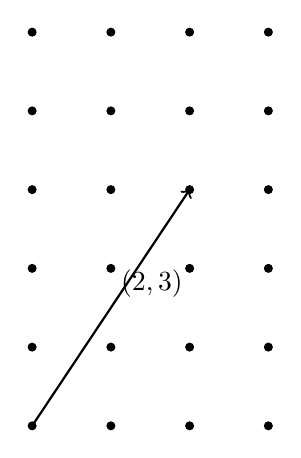
\begin{tikzpicture}
    \foreach \x in {0,1,2,3}
        \foreach \y in {0,1,2,3,4,5}
            \node[draw, circle, inner sep=1pt, fill=black] at (\x,\y) {};
    \draw[thick, ->] (0,0) -- (2,3) node[midway, above right] {$(2,3)$};
\end{tikzpicture}
\end{center}
    It is not hard to see that the line only intersect 2 points, so imagine 12 parrallel lines, which is the 12 cosets of G, so $G/H \cong \mathbb{Z}_{12}$ and the $G/H$ is cyclic.\\
    Now we use the first isomorphism theorem:\\
    Define \[\phi: \mathbb{Z}_4 \times \mathbb{Z}_6 \to \mathbb{Z}_{12} = \phi(a, b) = 3a - 2b\] 
    Then $\ker(\phi) = H$\\
    It is indeed a homomorphism because 
    \[\phi((a+c, b+d)) = 3(a+c) - 2(b+d) = 3a - 2b + 3c - 2d = \phi(a, b) + \phi(c, d)\]
    Thus by the first isomorphism theorem, $\mathbb{Z}_4 \times \mathbb{Z}_6 / \langle (2, 3) \rangle \cong \mathbb{Z}_{12}$.
\end{answer}

\begin{eg}
    $G = \mathbb{Z}_4 \times \mathbb{Z}_6$ and $H = \langle (0, 2) \rangle = \{(0, 0), (0, 2), (0, 4)\}$. Then $|G| = 24$ and $|H| = 3$. Thus $|G/H| = 24/3 = 8$.\\ 
    Now $G/H$ could be isomorphic to $\mathbb{Z}_8$ or $\mathbb{Z}_4 \times \mathbb{Z}_2$ or $\mathbb{Z}_2 \times \mathbb{Z}_2 \times \mathbb{Z}_2$.\\
\end{eg}
\begin{answer}
    Again, draw the lattice diagram, but we will omit here: intuitively, we see that $G/H \cong \mathbb{Z}_4 \times \mathbb{Z}_2$.\\
    Now we use the first isomorphism theorem:\\
    Define \[\phi(a, b) = (a, b\mod 2)\] 
    Then $\ker(\phi) = H$\\
    It is indeed a homomorphism because
    \[\phi((a+c, b+d)) = (a+c, b+d \mod 2) = (a, b \mod 2) + (c, d \mod 2) = \phi(a, b) + \phi(c, d)\]
    Thus by the first isomorphism theorem, $\mathbb{Z}_4 \times \mathbb{Z}_6 / \langle (0, 2) \rangle \cong \mathbb{Z}_4 \times \mathbb{Z}_2$.
\end{answer}